% asset_id: AS1QuadraticsTikZ-002
% source: CCEA AS1-AF-LO004 + discriminant lesson evidence
% related_section: Core Theory Part H – The Discriminant
% purpose: Three discriminant graph cases: D > 0, D = 0, D < 0.
\documentclass[tikz,border=8pt]{standalone}
\begin{document}
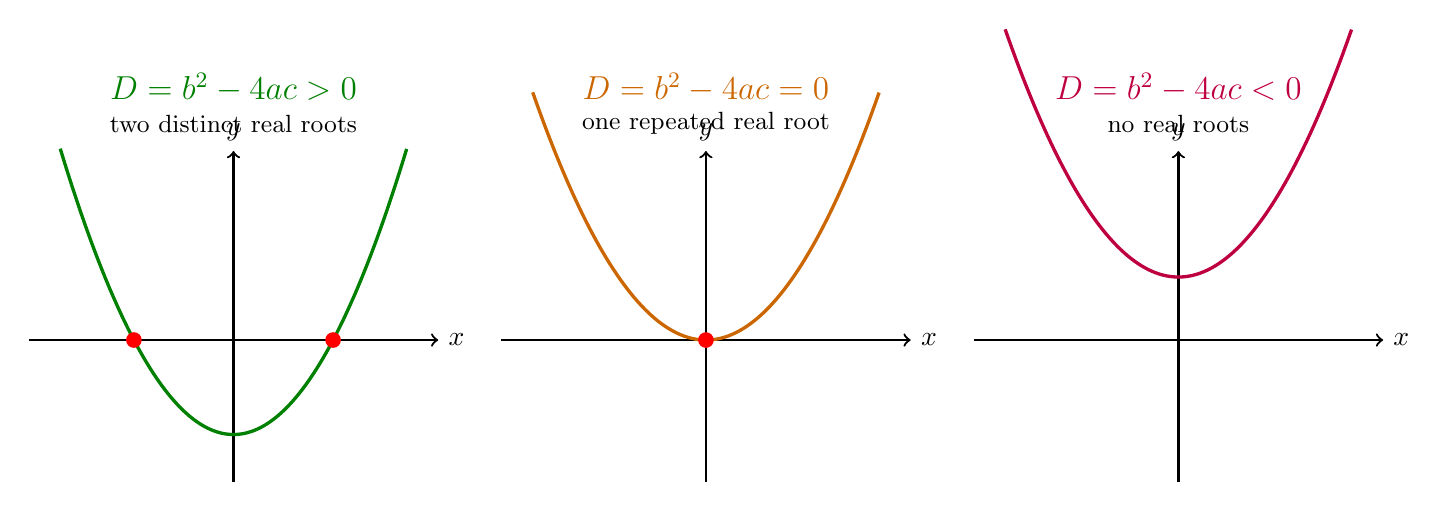
\begin{tikzpicture}[axis/.style={->, thick},curve/.style={very thick},point/.style={circle, fill=red, inner sep=2pt},title/.style={font=\bfseries\large},note/.style={font=\small, align=center}]
\begin{scope}[shift={(-6,0)}]
\node[title, green!50!black] at (0,3.2) {$D=b^2-4ac>0$}; \node[note] at (0,2.75) {two distinct real roots};
\draw[axis] (-2.6,0) -- (2.6,0) node[right] {$x$}; \draw[axis] (0,-1.8) -- (0,2.4) node[above] {$y$};
\draw[curve, green!50!black, domain=-2.2:2.2, samples=100] plot (\x,{0.75*\x*\x - 1.2});
\node[point] at (-1.265,0) {}; \node[point] at (1.265,0) {};
\end{scope}
\begin{scope}[shift={(0,0)}]
\node[title, orange!80!black] at (0,3.2) {$D=b^2-4ac=0$}; \node[note] at (0,2.75) {one repeated real root};
\draw[axis] (-2.6,0) -- (2.6,0) node[right] {$x$}; \draw[axis] (0,-1.8) -- (0,2.4) node[above] {$y$};
\draw[curve, orange!80!black, domain=-2.2:2.2, samples=100] plot (\x,{0.65*\x*\x}); \node[point] at (0,0) {};
\end{scope}
\begin{scope}[shift={(6,0)}]
\node[title, purple] at (0,3.2) {$D=b^2-4ac<0$}; \node[note] at (0,2.75) {no real roots};
\draw[axis] (-2.6,0) -- (2.6,0) node[right] {$x$}; \draw[axis] (0,-1.8) -- (0,2.4) node[above] {$y$};
\draw[curve, purple, domain=-2.2:2.2, samples=100] plot (\x,{0.65*\x*\x + 0.8});
\end{scope}
\end{tikzpicture}
\end{document}
